
\documentclass[english,a4paper]{article}

\usepackage[T1]{fontenc}
\usepackage[utf8]{inputenc}
\usepackage{lmodern}
\usepackage[a4paper,margin=0.85in]{geometry} % Réduire les marges
\usepackage[english]{babel}
\usepackage{amsmath}
\usepackage{amssymb}
\usepackage{amsthm}

\usepackage{cite} % Pour importer une bibliographie

\usepackage{bbm}
\usepackage{mathtools}
%\usepackage{ulem} % Pour barrer du texte
\usepackage{xcolor} % Pour colorer des symboles dans les équations

\usepackage{tikz} % Pour les dessins
\usepackage{enumitem} % Pour mettre des symboles au choix dans les énumérations
\usepackage{xfrac} % Pour faire des petites fractions : \sfrac{5}{7}

\usepackage{algorithm}
\usepackage{algpseudocode} % Pour écrire des algorithmes
\floatname{algorithm}{Algorithme} % ... en français


% Theorems
\theoremstyle{plain}
\newtheorem{theorem}{Théorème}
\newtheorem{proposition}{Proposition}
\newtheorem{lemma}{Lemme}
\newtheorem{corollary}{Corollaire}

\theoremstyle{definition}
\newtheorem{definition}{Définition}

\theoremstyle{remark}
\newtheorem{remark}{Remarque}
\newtheorem{example}{Exemple}


% Math operators
\newcommand{\scal}[2]{\left\langle #1 , #2 \right\rangle}
\DeclareMathOperator{\IR}{\mathbb{R}}
\DeclareMathOperator*{\argmin}{argmin}
\DeclareMathOperator*{\argmax}{argmax}
\DeclareMathOperator{\One}{\mathbbm{1}}
\DeclareMathOperator{\Ccal}{\mathcal{C}}
\DeclareMathOperator{\logsumexp}{logsumexp}
\DeclareMathOperator{\diag}{diag}
\DeclareMathOperator{\MAP}{MAP}

\newcommand{\norm}[1]{\left\lVert #1 \right\rVert}
\renewcommand{\epsilon}{\varepsilon}



\title{Mathematical foundations of data science\\
Blind deconvolution}
\date{January 2018}
\author{Alexis THIBAULT}

\begin{document}

\maketitle

\section{Abstract}
Blur is a common artifact in medical imagery, astronomy, microscopy, or even photography, which is generally undesirable as it obscures significant information.
In many cases the distortion can be modeled as a convolution, with an unknown kernel \cite{fergus2006removing,cho2009fast,cho2010motion,jia2007single,xu2010two}. One must therefore use \emph{blind deconvolution} to estimate the kernel, along with the de-blurred image.
Since there are more unknowns than data, the problem is ill-posed: assumptions are needed on the original image. The typical constraints are expressed as statistics on the distribution of the gradient \cite{joshi2008psf,krishnan2009fast,levi2009using,levin2007blind}, although more complex techniques have also been proposed \cite{miskin2000ensemble,jalobeanu2002satellite}. Here, we study the case of a Gaussian prior on the gradient, and show its limitations. We also consider adding a regularity prior on the kernel.
Blind deconvolution is often performed by alternating estimation of the blur kernel and the corresponding image, within a bayesian framework \cite{richardson1972bayesian,levin2007blind,levin2009understanding,levin2011efficient,krishnan2009fast,joshi2008psf,jia2007single,levi2009using}.
Here we use \emph{maximum a posteriori} ($\MAP$) estimation. We show numerically that, as explained in \cite{levin2011efficient}, maximizing the likelihood of the kernel ($\MAP_k$) before computing the image yields better results than estimating both image and kernel ($\MAP_{x,k}$).




\section{Introduction}
Many photographs taken without a tripod contain disappointing motion blur caused by camera shake. Such degradation is often approximately linear, and except in the special case when complex movement comes into play \cite{shan2007rotational,whyte2012non}, it is shift-invariant. The transformation of the image can thus be modeled as a convolution with a kernel.
In astronomy as well as microscopy, measuring tools often exhibit a wide \emph{point spread function} (PSF), which results in blurry images, in which significant data is obscured. This may be caused by atmospheric aberrations, or simply by diffraction.
In medical imagery \cite{chen2016compressive}, data acquired with compressive sensing often shows blur, which makes readings difficult.

In all these cases, we are interested in recovering an approximation of the original image, while being given only a distorted version of it:
\[
y = k * x + w.
\]
When the \emph{point spread function} (PSF) can be measured, as is sometimes the case in microscopy, the convolution kernel is known.
Restoring the original image is then a \emph{non-blind deconvolution problem}.
This simple inverse problem can be solved efficiently: in the absence of noise, one simply needs to apply the inverse filter in the Fourier domain.

Presence of noise makes things slightly more challenging.
Various image priors may be used \cite{sun2014good}.
A common form of image prior is obtained by conditioning on the derivatives. Let $(D_h x)_i$ and $(D_v x)_i$ denote the horizontal and vertical discrete derivatives of image $x$ at pixel $i$.
Take some model $\rho$ for the repartition of the derivatives, and set
\[
p(x) = \prod_i \rho((D_h x)_i) \rho((D_v x)_i) .
\]
Common settings for function $\rho$ are exponential of power functions \cite{krishnan2009fast,levin2009understanding}, and mixtures of Gaussians (MOG) \cite{levin2011efficient,fergus2006removing}.
A special case of these two is the Gaussian prior, which corresponds to $\rho(v) \propto e^{-\frac{|v|}{2\sigma^2}}$, and can be reformulated as an $L^2$-sparsity prior of the gradient. In that case one obtains Wiener deconvolution, which is linear, and may be computed very efficiently in the Fourier domain. However, this technique results in ringing artifacts around edges \cite{shan2008high}.
Using total variation better models the heavy-tail repartition of the derivatives in natural images \cite{chan1998total,levi2009using}.
More advanced methods have been devised for this problem \cite{sun2014good,schmidt2013discriminative}.



In most real-world cases, however, the kernel is unknown. This makes the problem of \emph{blind deconvolution} even more challenging.
Based on the blurry image, it aims at estimating both kernel and image.
Since the number of unknowns exceeds the data, the problem is ill-posed; it is therefore necessary to introduce assumptions about natural images.
Machine-learning oriented methods exist, such as learning the deblurring filter \cite{bell1995information}, but most commonly, a regularity prior on the image is used \cite{krishnan2009fast,fergus2006removing,levin2007blind,levi2009using,levin2011efficient,levin2009understanding,chan1998total}.
Again, it is often conditioned with the image derivatives, using various models. Wavelet sparsity priors have also been considered \cite{jalobeanu2002satellite}.

Blind deconvolution is commonly achieved by alternating estimation of the kernel and of the image.
This is usually done in a Bayesian framework: given an image distribution $p_x(x)$, a kernel distribution $p_k(k)$, and a noise distribution $p_w(w)$, find \emph{some likely explanation} $(x,k)$ of the observed image $y$ \cite{levin2009understanding,levin2011efficient}.
Several estimation strategies are available for choosing a \emph{likely explanation}. The direct one is to find a pair $(\hat{x},\hat{k})$ with maximal a posteriori probability \cite{cho2009fast,cho2007removing,jia2007single,shan2008high,xu2010two}.
As argued in \cite{levin2011efficient,levin2009understanding}, $\MAP_{x,k}$ estimation often leads to the no-blur explanation. The paper suggests to rather use $\MAP_k$ estimation, first finding the most likely kernel, then performing non-blind deconvolution \cite{fergus2006removing,whyte2012non}.

Whichever estimation is chosen, blind deconvolution is often performed by repeating two steps: kernel estimation, and image estimation \cite{jia2007single,fergus2006removing,levin2009understanding,levin2011efficient,shan2008high}. Some methods also include an additional `prediction' step \cite{cho2009fast}.

Here we consider deblurring images using both $\MAP_{x,k}$ and $\MAP_k$ algorithms, applied with a simple Gaussian prior. Using our own implementation, we show the results and the limitations of both. We also consider adding a Gaussian regularization prior on the kernel, leading to slight improvement.



\section{Method used}

\subsection{Problem}
Suppose we are given a distorted observation $y$ of a ground truth signal $x$, and we would like to recover x. The distortion is a convolution with an unknown kernel $k$, followed by the introduction of noise $w$.
\begin{equation}\label{eq:convolution}
y = k*x + w ,
\end{equation}
We will focus on the case when $x$ and $y$ are two-dimensional grids of pixels, but the methods can be easily generalized to higher dimensions. In particular, only the case of square images with $N = n\times n$ pixels will be treated.

\subsection{Priors}

Whether using $\MAP_{x,k}$ or $\MAP_k$, we are trying to maximize the likelihood of our guess. In order to do that, we need an \emph{a priori} probability distribution on $(x,y,k)$.
It is natural to suppose that $x$, $k$ and $w$ should be independent in formula (\ref{eq:convolution}). Everything is then characterized by the respective distributions of $x$, $k$ and $w$.

We suppose every pixel of $w$ to be independent Gaussian of variance $\eta^2$. Then, by substituting $w$ with $y-k*x$, we obtain:
\begin{equation}\label{eq:p_y|x,k}
p(y\mid x,k) = \frac{1}{(\eta\sqrt{2\pi})^N} e^{-\frac{1}{2\eta^2}\norm{k*x-y}^2} .
\end{equation}

Some model is also needed to characterize the kind of regularity we can suppose on the image.
If we were to choose a uniform image prior, then the best explanation would be absence of blur, i.e. with $x = y$ and $k$ being a single white pixel. But it makes sense to ensure some kind of regularity on the image, as some images are clearly more likely than others to appear as natural images.
For instance, we would like an image of a face, with zones having a smooth color gradient and with clear edges and lines and dots, to be more likely than white noise, or than the same image blurred.

Most image priors advantage some form of derivative sparsity\cite{krishnan2009fast, levin2009understanding, levin2011efficient, fergus2006removing}.
Let us denote by $(D_h x)_i$ (respectively $(D_v x)_i$) the horizontal (respectively vertical) gradient of $x$ at the $i$-th pixel. Then the formula goes:
\begin{equation}\label{eq:p_x_general}
p_x(x) = \prod_i \rho((D_h x)_i) \rho((D_v x)_i) .
\end{equation}
Then the prior is characterized by the choice of function $\rho$.
It is supposed to model the heavy-tail repartition of the gradient in natural images \cite{levi2009using} (see figure \ref{fig:heavytail}).
\begin{figure}
	\centering
	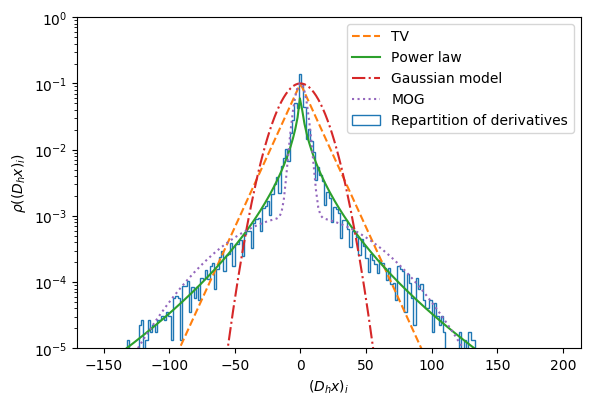
\includegraphics[width=10cm]{images/graph_derivatives}
	\caption{Various models for the repartition of gradients in natural images}
	\label{fig:heavytail}
\end{figure}
Function $\rho$ can take several forms in the literature.
\begin{itemize}
	\item The simplest alternative is a Gaussian prior \cite{levin2011efficient}:
	\begin{equation}\label{eq:rho_gaussian}
	\rho(v) = \frac{1}{\sigma \sqrt{2\pi}} \exp\left( -\frac{v^2}{2\sigma^2} \right) .
	\end{equation}
	When considering the log-likelihood, we see that this corresponds to an $L^2$-sparsity term on the gradient of $x$.
	\begin{align*}
	\log p_x(x) & = \frac{1}{2\sigma^2} \left( 
	\sum_i (D_h x)_i^2 
	+ \sum_i (D_v x)_i^2
	\right) + c\\
	& = \frac{1}{2\sigma^2} \norm{\nabla x}_2^2 +c ,
	\end{align*}
	where $c$ is some constant (we will use letter $c$ for denoting any constant additional term, with no dependence between equations).
	This prior is in fact a poor model of the repartition of derivatives. It encourages small values of the gradient, but forbids any large value to appear; whereas the actual repartition often features a heavy tail.
	Nevertheless, it is the one that will be used in numerics, as its analytical treatment allows for easier implementation.
	%
	%
	\item A slightly better model of the heavy-tail behavior penalizes the total variation---that is, the $L^1$ norm of the derivatives.
	\begin{equation}\label{eq:TV}
	\log p_x(x) \propto \sum_i |(\nabla x)_i|
	\end{equation}
	Replacing $|(\nabla x)_i|$ by $\norm{(\nabla x)_i}_1$ (if we neglect a factor between 1 and $\sqrt{2}$) allows us to approximate this in the form of equation (\ref{eq:p_x_general}), with:
	\begin{align*}
	\rho(v) = e^{-s|v|} .
	\end{align*}
	In this case, frequency-domain formulation is however not preferable, as it leads to a change in the norm of the gradient. Using $|D_h x| + |D_v x|$ instead of $\sqrt{|D_h x|^2 + |D_v x|^2}$ may result in artifacts exhibiting horizontal or vertical bias.
	%
	%
	\item One can also consider a `hyper-Laplacian' prior, where $\log \rho$ is a power law \cite{krishnan2009fast, levin2009understanding}:
	\begin{equation}\label{eq:p_hyper_laplacian}
	p_x(x) \propto \prod_i e^{-s|(\nabla x)_i|^\alpha}.
	\end{equation}
	Typical values of $\alpha$ are between 0.5 and 0.8, but $\alpha=2$ yields the Gaussian model, and $\alpha=1$ yields the total variation.
	However, this makes the problem non-convex.
	As before, we could be tempted to formulate things in the derivative-filter domain. We would set $\rho$ to be
	\begin{equation}\label{eq:rho_hyper_laplacian}
	\rho(v) \propto e^{-s|v|^\alpha}.
	\end{equation}
	Functions $\rho$ with this form very effectively model the heavy tail of the repartition, but using the derivative-filter formulation would lead to significant bias along the axes.
	%
	%
	\item A more general model, which can approximate more complex repartitions of derivatives, takes $\rho$ to be a \emph{mixture of gaussians} (MOG) \cite{fergus2006removing,levin2011efficient}:
	\begin{equation}\label{eq:rho_MOG}
	\rho(v) = \sum_j \frac{\pi_j}{\sigma_j\sqrt{2\pi}} e^{-\frac{v^2}{2\sigma_j^2}} .
	\end{equation}
	As explained in \cite{levin2011efficient}, this model is a good explanation for the features of images, and it allows to compute blind deconvolution by using hidden variables in the Expectation-Maximization algorithm to select which Gaussian component to use.
\end{itemize}


The kernel can often be assumed to have uniform density among kernels with positive values \cite{levi2009using}.
We also consider regularizing it with a Gaussian prior, as the kernels obtained in our algorithms tended to be very irregular.
\begin{equation}\label{eq:p_k_gaussian}
\log p(k) = -\frac{1}{2\sigma_k^2}\norm{\nabla k}_2^2
\end{equation}
Note that the smaller $\sigma_k$, the stronger the regularity. On the other hand, note that we can recover the uniform prior by setting $\sigma_k = +\infty$.


\subsection{Bayesian framework}
As discussed in \cite{levin2009understanding,levin2011efficient}, we consider two strategies for finding a good explanation of the observed image.
\begin{itemize}
	\item The older, more common, and more direct strategy is to estimate \emph{both} $x$ and $k$ at the same time, by maximizing their a posteriori probability \cite{cho2009fast,cho2007removing,jia2007single,shan2008high,xu2010two}.
	This is called $\MAP_{x,k}$ in \cite{levin2011efficient,levin2009understanding}, and is starkly criticized for often preferring the no-blur explanation.
	\begin{equation}\label{eq:MAP_xk}
	(\MAP_{x,k}) \quad\quad (\hat{x},\hat{k}) = \argmax_{x,k} p(x,k \mid y)
	\end{equation}
	%
	%
	\item The other approach presented in \cite{levin2009understanding} is the maximization of the a posteriori likelihood of the kernel ($\MAP_k$), with less regard to what the original image might be \cite{fergus2006removing,whyte2012non}.
	\begin{align}\label{eq:MAP_k}
	(\MAP_k) \quad\quad \hat{k} &= \argmax_{k} p(k \mid y)\\
	&= \argmax_{k} \int_x p(x,k \mid y) dx \nonumber .
	\end{align}
	This evaluation strategy less often falls for the no-blur explanation. However, it is more challenging, as the integral is difficult to compute.
\end{itemize}

In both cases, we can rewrite $p(x,k \mid y)$ in terms of our priors.
\begin{align*}
p(x,k \mid y) &\propto p(x,k,y)\\
&\propto p(y \mid x,k) p(x) p(k)\\
&\propto \exp\left( -\frac{\norm{k*x-y}^2}{2\eta^2} - \frac{\norm{\nabla k}^2}{2 \sigma_k^2}  \right) \prod_i \rho((D_h x)_i) \rho((D_v x)_i) .
\end{align*}
Posing the Gaussian prior on $\nabla x$, we even get
\begin{align*}
-\log p(x,k \mid y) &= \frac{\norm{k*x-y}^2}{2\eta^2} + \frac{\norm{\nabla k}^2}{2 \sigma_k^2} + \frac{\norm{\nabla x}^2}{2\sigma^2} + c .
\end{align*}
Note that the $\MAP_{x,k}$ estimator was ill-posed without kernel regularization: one could always take $(tk,x/t)$ for some solution, and get a better score by increasing $t$.
Our additional term counters this issue.

Despite the simple form of this prior, the nonlinearity introduced by the convolution makes it impossible to directly estimate $k$ and $x$ in a single step, even for $\MAP_{x,k}$. We therefore resolve to alternate estimation.


\subsection{Expectation-Maximization algorithm}
Both for $\MAP_{x,k}$ and $\MAP_k$, we will be using the Expectation-Maximization algorithm, which is a standard algorithm to compute $\MAP$ estimates.
Supposing $x$ is a hidden variable, the algorithm consists of two steps:
\begin{itemize}
	\item E-step:
	Given the observed image and an estimated kernel $k$, compute the first moments of the conditional probability distribution of $x$:
	\begin{equation}\label{eq:q}
	q(x) = p(x \mid k,y) .
	\end{equation}
	In the case of $\MAP_k$, one should compute both the mean $\mu$ \emph{and} the covariance $C$ of this distribution. For $\MAP_{x,k}$, the mean is sufficient, and set $C=0$.
	%
	%
	\item M-step:
	Considering a Gaussian approximation of the distribution of $x$,
	\[\tilde{q} = \mathcal{N}(\mu,C) ,\]
	compute the maximizer of the log-likelihood of $k$:
	\begin{align}\label{eq:M_step}
	\hat{k} 
	&= \argmax_k \int_x \log (p(y \mid x,k) p(k)) \tilde{q}(x) dx
	\\
	\label{eq:m_step_expectation}
	&= \argmin_k E_{\tilde{q}} \left[ \frac{\norm{k*x-y}^2}{2\eta^2} + \frac{\norm{\nabla k}^2}{2\sigma_k^2} \right]
	\end{align}	
\end{itemize}
This is an abstract formulation of the EM algorithm, but we will see that both steps can be rewritten in a more direct, numerics-oriented way.

\subsubsection{E-step: theory}
Thanks to the Gaussian prior on $\nabla x$, the computation of $\mu$ and $C$ is easily performed, as it reduces to a quadratic minimization problem.
If we expand the expression, and we regroup what is quadratic in $x$, and what is linear, we get the following:
\begin{align}\label{eq:e_step_quadratic}
-\log p(x \mid y,k) &= \frac{\norm{k*x-y}^2}{2\eta^2} + \frac{\norm{\nabla x}^2}{2\sigma^2} + c \nonumber
\\ 
&= \frac{1}{2}x^t A_x x - b_x x + c
\end{align}
with:
\begin{align*}
A_x &= \frac{1}{\eta^2} T_k^t T_k + \frac{1}{\sigma^2}(D_h^t D_h + D_v^t D_v)\\
b_x &= \frac{1}{\eta^2} T_k^t y
\end{align*}
where $T_k$ is the operator performing convolution with kernel $k$, and $D_h$ and $D_v$ are discrete differential operators, respectively along the horizontal and the vertical axis.

Recall the general formula for a Gaussian law of mean $\mu$ and covariance $C$, supposing $C$ is symmetric definite positive of size $N\times N$:
\begin{equation}\label{eq:general_gaussian}
p(x) = \frac{1}{(2\pi)^{\frac{N}{2}} \sqrt{\det C}} \exp \left( -\frac{(x-\mu)^t C^{-1} (x-\mu)}{2} \right) .
\end{equation}
Note that if we take
\begin{align}\label{eq:e_step_mu_and_C}
C &= A_x^{-1}
&
\mu = C b_x ,
\end{align}
then we can rewrite equation (\ref{eq:e_step_quadratic}) as:
\begin{equation}\label{eq:e_step_gaussian}
-\log p(x \mid y,k) = \frac{1}{2} (x-\mu)^t C^{-1} (x-\mu) + c
\end{equation}
This shows that distribution $p(x \mid y,k)$ is Gaussian, with mean $\mu$ and covariance $C$.
The formulas (\ref{eq:e_step_mu_and_C}) therefore define the correct mean and variance. They're what needs to be computed.


\subsubsection{E-step: in practice}
Note that operators $T_k$, $D_h$ and $D_v$, as they are convolutions, are diagonal in Fourier basis. Let us denote by $f_h$ and $f_v$ the convolution kernels corresponding to horizontal (respectively vertical) differentiation.
\begin{align}
T_k &= F^{-1} \diag(Fk) F\\
D_h &= F^{-1} \diag(Ff_h) F \nonumber \\
D_v &= F^{-1} \diag(Ff_v) F \nonumber \\
\label{eq:fourier_A_x}
F A_x F^{-1} &= \diag \left( \frac{|Fk|^2}{\eta^2} + \frac{|Ff_h|^2 + |Ff_v|^2}{\sigma^2} \right)
\end{align}
Therefore, the covariance is characterized by its diagonal in Fourier basis, which is the inverse of that of $A_x$. 

Note that $A_x$ is indeed invertible : $Ff_h$ is nonzero at all frequencies that contain horizontal variation, $Ff_v$ is nonzero at frequencies with vertical variation. Therefore $|Ff_h|^2 + |Ff_v|^2$ takes value zero only at the null frequency. Finally, the kernel has strictly positive mean, so that the complete sum in (\ref{eq:fourier_A_x}) has only positive coefficients.

In practice, it is possible to precompute $|Ff_h|^2+|Ff_v|^2$ (which are the eigenvalues of the Laplacian). We only need compute the diagonal $d_C$ of $C$ in Fourier basis (which is the pointwise inverse of that of $A_x$, and takes only one Fourier transform computation for $k$), and $\mu$ can be deduced.
\begin{align}\label{eq:mu_fourier}
\mu &= \frac{1}{\eta^2} C T_k^t y \nonumber\\
&= \frac{1}{\eta^2} F^{-1} \diag(d_C) \diag(\overline{Fk}) Fy \nonumber\\
\mu &= \frac{1}{\eta^2} F^{-1} (d_C \odot \overline{Fk} \odot Fy)
\end{align}
This shows that the computation of $\mu$ only uses two Fourier transforms (note that $Fk$ has already been computed) and some pointwise operations (on vectors of size $N$=number of pixels).

The Gaussian prior therefore has the advantage of allowing us to perform deconvolution with a very inexpensive process.
Note that, as it performs linear filtering on $y$, it is at best as good as Wiener deconvolution.

Note that the rescaling of the frequencies is in fact very similar to what is done in Wiener deconvolution. Given mean power spectral densities $K,X,W$ of $k,x$ and $w$ respectively, the optimal linear filter to restore the original image has spectral power density:
\begin{equation}\label{eq:wiener_deconv}
G = \frac{\overline{K}}{|K|^2 + \frac{W}{X}}
\end{equation}
Considering the expressions above, the Gaussian prior performs Wiener deconvolution, with 
\begin{align*}
K &= Fk,& W &= \eta^2,& X &= \frac{\sigma^2}{|Ff_h|^2+|Ff_v|^2}.
\end{align*}
Although it is very efficiently computed, this deconvolution thus suffers from the limitations of linear filters, and introduces ringing artifacts around edges \cite{shan2008high}.


\subsubsection{M-step: theory}

Let us expand and regroup quadratic and linear terms in (\ref{eq:m_step_expectation}).
\begin{align*}
\hat{k} = \argmin E_{\tilde{q}} \left[
\frac{1}{2} k^t A_k k - b_k k
\right].
\end{align*}
In the expression above, $A_k$ and $b_k$ depend on $x$ and $y$, with quadratic terms involving $x^2$ stemming from the convolution, and linear terms related to the expansion of the difference. The Gaussian prior leads to additional differentiation-related terms.
They can be expressed as follows:
\begin{align}
\label{eq:m_step_A_k}
A_k(i_1,i_2) &= \sum_i x(i+i_1) x(i+i_2) + \left(\frac{D_h^tD_h + D_v^tD_v}{\sigma_k^2} \right)(i_1,i_2) ,\\
\label{eq:m_step_b_k}
b_k(i_1) &= \sum_i x(i+i_1) y(i) .
\end{align}
If we consider windows of $x$ to represent observations of a random variable, then $A_k$ corresponds to a covariance matrix within these windows.

Taking the expectation relative to $x$ yields:
\begin{equation}\label{eq:m_step_quadratic}
\hat{k} = \argmin_k \frac{1}{2} k^t \bar{A_k} k - \bar{b_k} k,
\end{equation}
where the mean values $ \bar{A_k}$ and $ \bar{b_k}$ are
\begin{align}
\bar{A_k}(i_1,i_2)  &= \sum_i \mu(i+i_1)\mu(i+i_2) + \sum_i C(i+i_1,i+i_2) + \left(\frac{D_h^tD_h + D_v^tD_v}{\sigma_k^2} \right)(i_1,i_2) \\
\bar{b_k}(i_1) &= \sum_i \mu(i+i_1) y(i)
\end{align}

Hence the M-step can simply be rewritten as a quadratic programming problem:
\begin{equation}
\hat{k} = \argmin_k \frac{1}{2} k^t \bar{A_k} k - \bar{b_k} k \quad \quad \text{s.t. } k\ge 0 .
\end{equation}
The constraint $k\ge 0$ prevents analytic solution of the minimization problem in general.

\subsubsection{M-step: in practice}
Once again, formulation in Fourier domain can help us in order to simplify computations.
Let us consider that Fourier transform is written as
\begin{equation}\label{eq:fourier_mu}
\mu(i) = \frac{1}{\sqrt{N}} \sum_{f} \hat{\mu}(f) e^{\scal{f}{i}}.
\end{equation}

\begin{itemize}
	\item The first term in $\bar{A_k}(i_1,i_2)$ can be given a computable form:
\begin{align*}
\sum_i \mu(i+i_1)\mu(i+i_2) &= \frac{1}{N} \sum_f \sum_g \hat{\mu}(f) \hat{\mu}(g) \sum_i  e^{\scal{f}{i+i_1} + \scal{g}{i+i_2}}\\
&=\sum_f \sum_g \hat{\mu}(f) \hat{\mu}(g) e^{\scal{f}{i_1}+\scal{g}{i_2}}  \One_{\{f+g=0\}}\\
&= \sum_f \hat{\mu}(f) \hat{\mu}(-f) e^{\scal{f}{i_1-i_2}} .
\end{align*}
This term can be seen as the inverse Fourier transform of $\hat{\mu} \odot \tilde{\hat{\mu}}$, where $\tilde{\hat{\mu}}(f) = \hat{\mu}(-f)$. Since $\hat{\mu}$ was found in the E-step, this is a straightforward numerical computation.

	\item The second term can also be rewritten, based on the fact that $C$ is diagonal in Fourier basis:
\begin{align*}
C &= F^{-1} \diag(d_C) F\\
\sum_\ell C(\ell+i_1,\ell+i_2) 
&= \sum_\ell (F^{-1} \diag(d_C) F)(\ell+i_1,\ell+i_2)\\
&= \sum_\ell \sum_j F^{-1}(\ell+i_1,j) (\diag(d_C) F)(j,\ell+i_2)\\
&= \sum_\ell \sum_j d_C(j) F^{-1}(\ell+i_1,j) F(j,\ell+i_2)\\
&= \sum_j d_C(j)  \sum_\ell \frac{1}{\sqrt{N}} e^{-\frac{2i\pi}{n} \scal{\ell+i_1}{j}} \frac{1}{\sqrt{N}} e^{\frac{2i\pi}{n} \scal{\ell+i_2}{j}}\\
&= \sum_j d_C(j) e^{\frac{2i\pi}{n} \scal{i_2-i_1}{j}}\\
&= \sum_j F(i_2-i_1,j) d_C(j)\\
&= (F d_C)(i_2-i_1) .
\end{align*}
The coefficients $d_C$ were already computed in the E-step, so a simple Fourier transform directly gives the result.
Of course, this term only appears in the case of $\MAP_k$. For $\MAP_{x,k}$, it is simply absent.

	\item As in the E-step, the third term is the Laplacian matrix, which can efficiently be precomputed in Fourier domain.
	
	\item The expression of $\bar{b_k}$ can also be simplified. Calculations similar to those above lead to
	\begin{equation}\label{eq:b_k_fourier}
	\sum_i \mu(i+i_1) y(i) = \sum_f \hat{\mu}(f) \hat{y}(-f) e^{\scal{f}{i_1}} .
	\end{equation}
	Here again, this is performed with a single Fourier transform, as $\hat{\mu}$ and $\hat{y}$ were computed in the E-step.
\end{itemize}


Since the kernel size is generally not too big ($15\times 15$ in our implementation), once $\bar{A_k}$ and $\bar{b_k}$ are computed a simple quadratic solver gives the solution in a short amount of time.



\subsubsection{TODO Theoretical guarantee: likelihood increase?}
% TODO Theoretical guarantee ?


\section{Numerical results}
I implemented the EM algorithm with Gaussian prior in \texttt{python}, using \texttt{numpy} for efficient computation and \texttt{scipy.optimize} for quadratic optimization in the M-step.
The results are presented in figures \ref{fig:results_louxor}-\ref{fig:results_candy}.


    \begin{figure}
    \centering
    \begin{tabular}{c c c}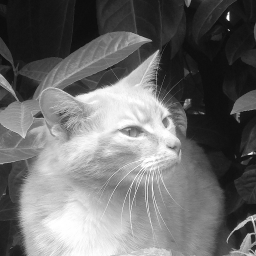
\includegraphics[width=4cm]{images/louxor} 
& 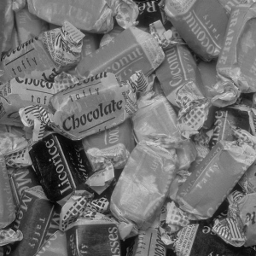
\includegraphics[width=4cm]{images/chocolate} 
& 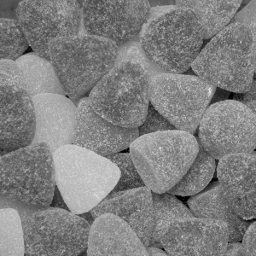
\includegraphics[width=4cm]{images/candy} 
\\ 
\texttt{louxor} 
& \texttt{chocolate} 
& \texttt{candy} 

    \end{tabular}
    \begin{tabular}{c c c c}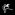
\includegraphics[width=2cm]{images/kernel1} 
& 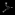
\includegraphics[width=2cm]{images/kernel2} 
& 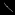
\includegraphics[width=2cm]{images/kernel3} 
& 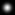
\includegraphics[width=2cm]{images/kernelgauss} 
\\ 
\texttt{kernel1} 
& \texttt{kernel2} 
& \texttt{kernel3} 
& \texttt{kernelgauss} 

\end{tabular}
\caption{Images and kernels used in our tests}
\end{figure}
    \begin{figure}
    \centering
    \begin{tabular}{|l|l|l|l|l|l|}
 \hline 
Blurred & Non-blind & $\MAP_{x,k}$ & $\MAP_k$, $\sigma_k=+\infty$ & Regularized $\MAP_k$ \\ 
 \hline 
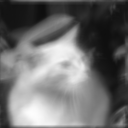
\includegraphics[width=2.5cm]{results/louxor_kernel1_blurred.png}
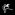
\includegraphics[width=0.5cm]{images/kernel1}
& 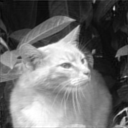
\includegraphics[width=2.5cm]{results/louxor_kernel1_nonblind_deconv.png}
&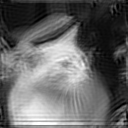
\includegraphics[width=2.5cm]{results/louxor_kernel1_MAPxk_x.png}
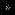
\includegraphics[width=0.5cm]{results/louxor_kernel1_MAPxk_k.png}
&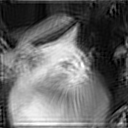
\includegraphics[width=2.5cm]{results/louxor_kernel1_MAPk_x.png}
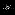
\includegraphics[width=0.5cm]{results/louxor_kernel1_MAPk_k.png}
&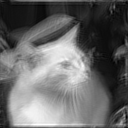
\includegraphics[width=2.5cm]{results/louxor_kernel1_MAPkreg_x.png}
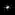
\includegraphics[width=0.5cm]{results/louxor_kernel1_MAPkreg_k.png}
\\ 
 \hline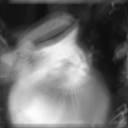
\includegraphics[width=2.5cm]{results/louxor_kernel2_blurred.png}
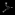
\includegraphics[width=0.5cm]{images/kernel2}
& 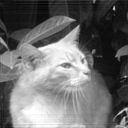
\includegraphics[width=2.5cm]{results/louxor_kernel2_nonblind_deconv.png}
&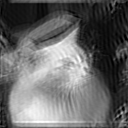
\includegraphics[width=2.5cm]{results/louxor_kernel2_MAPxk_x.png}
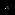
\includegraphics[width=0.5cm]{results/louxor_kernel2_MAPxk_k.png}
&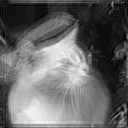
\includegraphics[width=2.5cm]{results/louxor_kernel2_MAPk_x.png}
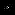
\includegraphics[width=0.5cm]{results/louxor_kernel2_MAPk_k.png}
&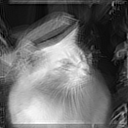
\includegraphics[width=2.5cm]{results/louxor_kernel2_MAPkreg_x.png}
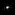
\includegraphics[width=0.5cm]{results/louxor_kernel2_MAPkreg_k.png}
\\ 
 \hline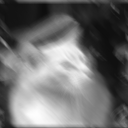
\includegraphics[width=2.5cm]{results/louxor_kernel3_blurred.png}
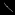
\includegraphics[width=0.5cm]{images/kernel3}
& 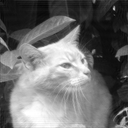
\includegraphics[width=2.5cm]{results/louxor_kernel3_nonblind_deconv.png}
&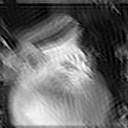
\includegraphics[width=2.5cm]{results/louxor_kernel3_MAPxk_x.png}
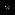
\includegraphics[width=0.5cm]{results/louxor_kernel3_MAPxk_k.png}
&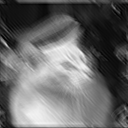
\includegraphics[width=2.5cm]{results/louxor_kernel3_MAPk_x.png}
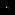
\includegraphics[width=0.5cm]{results/louxor_kernel3_MAPk_k.png}
&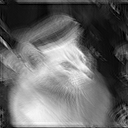
\includegraphics[width=2.5cm]{results/louxor_kernel3_MAPkreg_x.png}
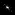
\includegraphics[width=0.5cm]{results/louxor_kernel3_MAPkreg_k.png}
\\ 
 \hline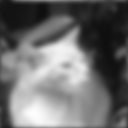
\includegraphics[width=2.5cm]{results/louxor_kernelgauss_blurred.png}
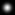
\includegraphics[width=0.5cm]{images/kernelgauss}
& 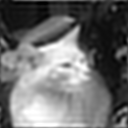
\includegraphics[width=2.5cm]{results/louxor_kernelgauss_nonblind_deconv.png}
&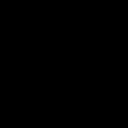
\includegraphics[width=2.5cm]{results/louxor_kernelgauss_MAPxk_x.png}
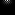
\includegraphics[width=0.5cm]{results/louxor_kernelgauss_MAPxk_k.png}
&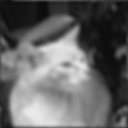
\includegraphics[width=2.5cm]{results/louxor_kernelgauss_MAPk_x.png}
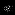
\includegraphics[width=0.5cm]{results/louxor_kernelgauss_MAPk_k.png}
&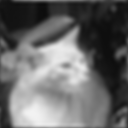
\includegraphics[width=2.5cm]{results/louxor_kernelgauss_MAPkreg_x.png}
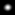
\includegraphics[width=0.5cm]{results/louxor_kernelgauss_MAPkreg_k.png}
\\ 
 \hline\end{tabular} 

    \caption{Results on \texttt{louxor} image}\label{fig:results_louxor}
    \end{figure}
    \begin{figure}
    \centering
    \begin{tabular}{|l|l|l|l|l|l|}
 \hline 
Blurred & Non-blind & $\MAP_{x,k}$ & $\MAP_k$, $\sigma_k=+\infty$ & Regularized $\MAP_k$ \\ 
 \hline 
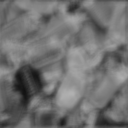
\includegraphics[width=2.5cm]{results/chocolate_kernel1_blurred.png}
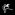
\includegraphics[width=0.5cm]{images/kernel1}
& 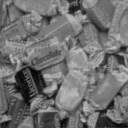
\includegraphics[width=2.5cm]{results/chocolate_kernel1_nonblind_deconv.png}
&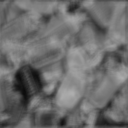
\includegraphics[width=2.5cm]{results/chocolate_kernel1_MAPxk_x.png}
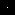
\includegraphics[width=0.5cm]{results/chocolate_kernel1_MAPxk_k.png}
&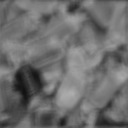
\includegraphics[width=2.5cm]{results/chocolate_kernel1_MAPk_x.png}
\includegraphics[width=0.5cm]{results/chocolate_kernel1_MAPk_k.png}
&\includegraphics[width=2.5cm]{results/chocolate_kernel1_MAPkreg_x.png}
\includegraphics[width=0.5cm]{results/chocolate_kernel1_MAPkreg_k.png}
\\ 
 \hline\includegraphics[width=2.5cm]{results/chocolate_kernel2_blurred.png}
\includegraphics[width=0.5cm]{images/kernel2}
& \includegraphics[width=2.5cm]{results/chocolate_kernel2_nonblind_deconv.png}
&\includegraphics[width=2.5cm]{results/chocolate_kernel2_MAPxk_x.png}
\includegraphics[width=0.5cm]{results/chocolate_kernel2_MAPxk_k.png}
&\includegraphics[width=2.5cm]{results/chocolate_kernel2_MAPk_x.png}
\includegraphics[width=0.5cm]{results/chocolate_kernel2_MAPk_k.png}
&\includegraphics[width=2.5cm]{results/chocolate_kernel2_MAPkreg_x.png}
\includegraphics[width=0.5cm]{results/chocolate_kernel2_MAPkreg_k.png}
\\ 
 \hline\includegraphics[width=2.5cm]{results/chocolate_kernel3_blurred.png}
\includegraphics[width=0.5cm]{images/kernel3}
& \includegraphics[width=2.5cm]{results/chocolate_kernel3_nonblind_deconv.png}
&\includegraphics[width=2.5cm]{results/chocolate_kernel3_MAPxk_x.png}
\includegraphics[width=0.5cm]{results/chocolate_kernel3_MAPxk_k.png}
&\includegraphics[width=2.5cm]{results/chocolate_kernel3_MAPk_x.png}
\includegraphics[width=0.5cm]{results/chocolate_kernel3_MAPk_k.png}
&\includegraphics[width=2.5cm]{results/chocolate_kernel3_MAPkreg_x.png}
\includegraphics[width=0.5cm]{results/chocolate_kernel3_MAPkreg_k.png}
\\ 
 \hline\includegraphics[width=2.5cm]{results/chocolate_kernelgauss_blurred.png}
\includegraphics[width=0.5cm]{images/kernelgauss}
& \includegraphics[width=2.5cm]{results/chocolate_kernelgauss_nonblind_deconv.png}
&\includegraphics[width=2.5cm]{results/chocolate_kernelgauss_MAPxk_x.png}
\includegraphics[width=0.5cm]{results/chocolate_kernelgauss_MAPxk_k.png}
&\includegraphics[width=2.5cm]{results/chocolate_kernelgauss_MAPk_x.png}
\includegraphics[width=0.5cm]{results/chocolate_kernelgauss_MAPk_k.png}
&\includegraphics[width=2.5cm]{results/chocolate_kernelgauss_MAPkreg_x.png}
\includegraphics[width=0.5cm]{results/chocolate_kernelgauss_MAPkreg_k.png}
\\ 
 \hline\end{tabular} 

    \caption{Results on \texttt{chocolate} image}\label{fig:results_chocolate}
    \end{figure}
    \begin{figure}
    \centering
    \begin{tabular}{|l|l|l|l|l|l|}
 \hline 
Blurred & Non-blind & $\MAP_{x,k}$ & $\MAP_k$, $\sigma_k=+\infty$ & Regularized $\MAP_k$ \\ 
 \hline 
\includegraphics[width=2.5cm]{results/candy_kernel1_blurred.png}
\includegraphics[width=0.5cm]{images/kernel1}
& \includegraphics[width=2.5cm]{results/candy_kernel1_nonblind_deconv.png}
&\includegraphics[width=2.5cm]{results/candy_kernel1_MAPxk_x.png}
\includegraphics[width=0.5cm]{results/candy_kernel1_MAPxk_k.png}
&\includegraphics[width=2.5cm]{results/candy_kernel1_MAPk_x.png}
\includegraphics[width=0.5cm]{results/candy_kernel1_MAPk_k.png}
&\includegraphics[width=2.5cm]{results/candy_kernel1_MAPkreg_x.png}
\includegraphics[width=0.5cm]{results/candy_kernel1_MAPkreg_k.png}
\\ 
 \hline\includegraphics[width=2.5cm]{results/candy_kernel2_blurred.png}
\includegraphics[width=0.5cm]{images/kernel2}
& \includegraphics[width=2.5cm]{results/candy_kernel2_nonblind_deconv.png}
&\includegraphics[width=2.5cm]{results/candy_kernel2_MAPxk_x.png}
\includegraphics[width=0.5cm]{results/candy_kernel2_MAPxk_k.png}
&\includegraphics[width=2.5cm]{results/candy_kernel2_MAPk_x.png}
\includegraphics[width=0.5cm]{results/candy_kernel2_MAPk_k.png}
&\includegraphics[width=2.5cm]{results/candy_kernel2_MAPkreg_x.png}
\includegraphics[width=0.5cm]{results/candy_kernel2_MAPkreg_k.png}
\\ 
 \hline\includegraphics[width=2.5cm]{results/candy_kernel3_blurred.png}
\includegraphics[width=0.5cm]{images/kernel3}
& \includegraphics[width=2.5cm]{results/candy_kernel3_nonblind_deconv.png}
&\includegraphics[width=2.5cm]{results/candy_kernel3_MAPxk_x.png}
\includegraphics[width=0.5cm]{results/candy_kernel3_MAPxk_k.png}
&\includegraphics[width=2.5cm]{results/candy_kernel3_MAPk_x.png}
\includegraphics[width=0.5cm]{results/candy_kernel3_MAPk_k.png}
&\includegraphics[width=2.5cm]{results/candy_kernel3_MAPkreg_x.png}
\includegraphics[width=0.5cm]{results/candy_kernel3_MAPkreg_k.png}
\\ 
 \hline\includegraphics[width=2.5cm]{results/candy_kernelgauss_blurred.png}
\includegraphics[width=0.5cm]{images/kernelgauss}
& \includegraphics[width=2.5cm]{results/candy_kernelgauss_nonblind_deconv.png}
&\includegraphics[width=2.5cm]{results/candy_kernelgauss_MAPxk_x.png}
\includegraphics[width=0.5cm]{results/candy_kernelgauss_MAPxk_k.png}
&\includegraphics[width=2.5cm]{results/candy_kernelgauss_MAPk_x.png}
\includegraphics[width=0.5cm]{results/candy_kernelgauss_MAPk_k.png}
&\includegraphics[width=2.5cm]{results/candy_kernelgauss_MAPkreg_x.png}
\includegraphics[width=0.5cm]{results/candy_kernelgauss_MAPkreg_k.png}
\\ 
 \hline\end{tabular} 

    \caption{Results on \texttt{candy} image}\label{fig:results_candy}
    \end{figure}


The images used are of size $128\times 128$ pixels, blurred with artificially-generated kernels of size $15\times 15$. The parameters used are $\sigma = 0.3$, and in the case of kernel-regularized $\MAP_k$, $\sigma_k = 6.10^{-5}$ (for larger values of $\sigma_k$ the regularization had too little effect).

In order to avoid dwelling on the no-blur explanation, and to speed up convergence, we use decreasing values of $\eta$ during the algorithm. It is initialized to $1$, and multiplied by $0.7$ until it gets below $0.01$.


As can be seen, the Gaussian prior shows serious limitations.
\begin{itemize}
	\item The first issue, though not the worst, is caused by the linear filtering in our M-step, which means the best possible result is given by non-blind Wiener deconvolution.
	Although for most kernels the issue is not too serious, when we use a Gaussian kernel, which strongly attenuates high frequencies, the Wiener filter is unable to restore them.
	For all three images, the best possible result of our algorithm will in any case be blurry and exhibit ringing around edges.
	
	\item In all cases, we see that the $\MAP_{x,k}$ estimator completely fails at removing the blur, simply because it often does not even try.
	In 4 cases out of 12, it finds that the image has not been blurred at all. In another case, it even diverges.
	In the cases when it tries something, the result most often very similar to the blurred image, only with more ringing.
	
	This illustrates the point made in \cite{levin2009understanding}, that the $\MAP_{x,k}$ estimation strategy fails to deblur images, because it favors the no-blur explanation.
	
	\item The $\MAP_k$ approach (without kernel regularization) is the one suggested as a better alternative to $\MAP_{x,k}$ in \cite{levin2009understanding}.
	In our tests, however, its results are comparable to those of $\MAP_{x,k}$.
	It also favors the no-blur explanation in 4 cases out of 12 (which are not the same, interestingly).
	The best results of $\MAP_k$ are still disappointing, however, as it does not succeed once at giving a good deblurring result.
	The difference with the previous method is, however, that it does not result in as much ringing. Moreover, when it tries something, it goes in the right direction: for instance, on images \texttt{chocolate} and \texttt{candy} with the third kernel, $\MAP_k$ figured out that something was going on in the diagonal direction, but it just aligned a few dots and was not able to give a regular enough kernel.
	In other cases the estimated kernel was also composed of a few isolated dots, which is rarely a good estimation.
	
	\item This erratic roughness in the obtained kernels led to the idea of giving the kernel a bias towards more regularity. Adding a Gaussian prior to the kernel only adds the last term to equation (\ref{eq:m_step_A_k}), and does not significantly change the necessary computations.
	
	Using $\MAP_k$ with this kernel regularization leads to slight improvement in the results. The no-blur explanation is no longer favored, since it induces a strong gradient in the kernel: all results are at least a bit smooth.
	
	Whenever \texttt{kernelgauss} was used, the algorithm successfully found that the kernel was a smooth spot, and the failure of the deblurring mainly comes from the linear filtering approach.
	
	Results from using \texttt{kernel3} all feature a diagonally-oriented line of positive coefficients. However, coefficients in the middle of the image are much larger than the others, resulting in only partial restoration. Instead of a mixture of continuously translated images, it now looks like a mixture of just two; which is better, but not perfect.
	
	Another improvement is found in the restoration of textures: in spite of the low fidelity of the Gaussian prior, the images recovered by kernel-regularized-$\MAP_k$ are sometimes much sharper (although still visibly distorted) than those with non-kernel-regularized-$\MAP_k$.
	Good examples are found by looking at textures in the restored versions of image \texttt{candy}. The sugary texture on the surface of the candy is more accurately restored by kernel regularization.
	
	
\end{itemize}


\section{Conclusion}

Blind deconvolution with a Gaussian prior as presented in \cite{levin2009understanding,levin2011efficient} was generalized for using kernel regularization, and implemented in \texttt{python}.

The tests, performed on $128\times 128$ images, show the limitations of the Gaussian prior: none of the original images was faithfully recovered.
However, they still show significant difference between the different possible approaches, which are $\MAP_{x,k}$, $\MAP_k$ without kernel regularization, and $\MAP_k$ with kernel regularization.

The Gaussian prior allows for simple computation: numerics are very efficiently performed in the Fourier domain. However, this prior does not faithfully model the repartition of gradients in natural images. In particular, edges are given a low score, and smooth gradients are preferred. It is therefore no wonder that the results obtained are disappointing.

Using a non-uniform prior on the kernel (namely, a Gaussian prior on its derivatives) is possible at low computational cost, since it simply adds a Laplacian term to the quadratic minimization problem that needs to be solved.

Difficulty in implementing the Gaussian prior deterred me from testing more complicated models, but the mixture of Gaussians model would have similar basic steps and get much better results \cite{levin2011efficient}.

One observation that could be made from the tests is that using kernel regularization does slightly improve the overall results of Gaussian-prior $\MAP_k$. 
Maybe using kernel regularization could lead to improvement in more advanced models as well. 
It is clear that in photography, some camera shake kernels are more likely than others: finding a good prior could probably help improve the accuracy of deblurring methods.


\bibliographystyle{plain}
\bibliography{references}

\end{document}
